%% \begin{tikzpicture}

%%     \tikzstyle{region} = [rounded corners, fill]

%%     \colorlet{red}{red!50}
%%     \colorlet{blue}{blue!50}
%%     \colorlet{green}{green!50}

%%     \draw[line width=1, ->] (0,0) -- (5,0) node[below] {\large observable 1};
%%     \draw[line width=1, ->] (0,0) -- (0,5) node[left, rotate=90] {\large observable 2};

%%     %\draw[dashed, line width=0.8] (5, 0) -- (5, 7);
%%     %\draw node at (5,-0.3) {\large $t_c$};

%%     %\draw node at (1.5, 4) {\large $g(t|H_0)$};

%%     \draw[region, red] (0.2,0.2) rectangle (1.6,1.6) node[midway,black] {CR};

%%     \draw[region, green] (3.2,3.2) rectangle (4.9,4.9) node[midway,black] {SR};

%%     \draw[region, blue] (1,2) rectangle (4.9,3) node[midway,black] {VR};
%%     \draw[region, blue] (1,3.1) rectangle (3,4.9) node[midway,black] {VR};


%%     %\draw node (alpha) at (3,-0.5) {\large $\beta$};
%%     %\draw node (p0) at (4.7,0.5) {};
%%     %\draw[->] (p0) edge[bend left] (alpha);

%%     %\draw node (beta) at (7,-0.5) {\large $\alpha$};
%%     %\draw node (p1) at (5.1,0.2) {};
%%     %\draw[->] (p1) edge[bend right] (beta);

%% \end{tikzpicture}

%% \usetikzlibrary{positioning}

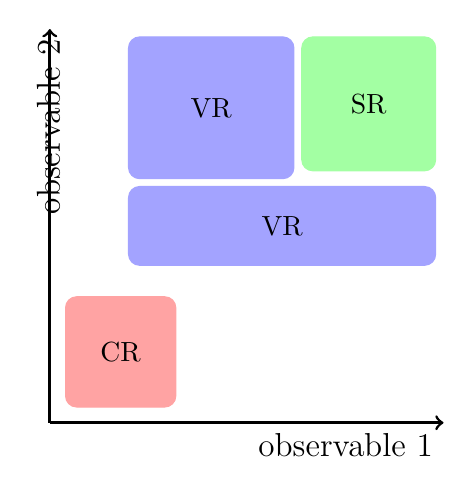
\begin{tikzpicture}

  \tikzstyle{region} = [rounded corners, fill]

  \colorlet{red}{red!60}
  \colorlet{blue}{blue!60}
  \colorlet{green}{green!60}

  \draw[line width=1, ->] (0,0) -- (5,0) node[below left] {\large observable 1};
  \draw[line width=1, ->] (0,0) -- (0,5) node[left=0.5,rotate=90] {\large observable 2};

  %\draw[dashed, line width=0.8] (5, 0) -- (5, 7);
  %\draw node at (5,-0.3) {\large $t_c$};

  \draw[region, red] (0.2,0.2) rectangle (1.6,1.6) node[midway,black] {CR};

  \draw[region, green] (3.2,3.2) rectangle (4.9,4.9) node[midway,black] {SR};

  \draw[region, blue] (1,2) rectangle (4.9,3) node[midway,black] {VR};
  \draw[region, blue] (1,3.1) rectangle (3.1,4.9) node[midway,black] {VR};

  %\draw node (alpha) at (3,-0.5) {\large $\beta$};
  %\draw node (p0) at (4.7,0.5) {};
  %\draw[->] (p0) edge[bend left] (alpha);

  %\draw node (beta) at (7,-0.5) {\large $\alpha$};
  %\draw node (p1) at (5.1,0.2) {};
  %\draw[->] (p1) edge[bend right] (beta);

\end{tikzpicture}
